\section{Introduction}

\begin{frame}
	\begin{block}{Fair AI Similarity Search (\texttt{faiss})}
		In this report, we cover results of our experiments with \texttt{faiss}\footnotemark \, library \cite{Johnson2017} powered by GPU\footnotemark \, for the nearest neighbors search. The report includes the following:
		\begin{itemize}
			\item Timing comparison for the k-means task on SIFT2M data evaluated before;
			\item k-NN graph construction with various indices from \texttt{faiss} and evaluation of timings and precision on Oxford105K data set.
			\item Implementation of the smooth path algorithm within the k-NN graph based on (12) of \cite{Johnson2017}. Oxford105K data was utilized.
		\end{itemize}
	\end{block}
	
	\begin{block}{Technical Details}
		The respective implementation is available on our \href{https://github.com/salisaresama/computer-vision}{{\color{blue}\underline{GitHub}}} page.
	\end{block}
	
	\addtocounter{footnote}{-2}
	\stepcounter{footnote}\footnotetext{Link to the Fair AI Similarity Search library we used: \href{https://github.com/facebookresearch/faiss}{{\color{blue}\underline{faiss}}}.}
	\stepcounter{footnote}\footnotetext{NVIDIA GTX 1080Ti}
\end{frame}


\section{$k$-means Task}
\subsection{Timing}


\begin{frame}

\begin{block}{$k$-means Exercise Revisited with GPU}

Once again we perform naive $k$-means iterations on the SIFT2M data set with $k = 32000$. However, this time during each iteration only exact nearest neighbors are searched for. Moreover, the search is done by means of GPU. As expected, the \texttt{IndexFlatL2} index from \texttt{faiss} on a GPU-enabled machine performs the search of nearest cluster centers more than a thousand times faster (recall that it took approx. 9K seconds before). Cluster assignment still takes relatively long, as it was not optimized for GPU by us.
	
\end{block}


	\begin{table}
		\small
		\begin{tabular}{| c || c | c |}
			\hline
			Title & (AVG. | STD.) NN time, [s] & (AVG. | STD.) cluster assignment time, [s] \\
			\hline
			\hline			
			$k$-means iteration & 2.58 | 0.37 & 136.56 | 18.36 \\
			\hline  
		\end{tabular}
	\end{table}
\end{frame}


\section{k-NN Graph}
\subsection{Description}

\begin{frame}

\begin{block}{$k$-NN Graph Construction with GPU}

	We also used the power of GPU and \texttt{faiss} to construct $k$-NN graphs. A few indices were tried out: \texttt{IndexFlatL2} (exhaustive searches), \texttt{IndexIVFFlat} (non-exhaustive searches with inverted indices), and \texttt{IndexIVFPQ} (product quantization powered with a coarse quantizer). The table below contains fixed parameters used to measure both timings to construct $k$-NN graphs and precision of results:

\begin{itemize}
	\item Fig.~\ref{fig:knn_timing} demonstrates timings dependent on the query size (note that the current GPU-enabled implementation of \texttt{faiss} (version 1.6.3) only scales up to 1024 neighbors per query);
	\item Fig.~\ref{fig:knn_precision} showcases performance of \texttt{IndexIVFFlat} and \texttt{IndexIVFPQ}. To estimate performance, we measure recall which is calculated as the average fraction over queries (all images from the data set) of first $k$ true nearest neighbors found during the search of $K$ approximate nearest neighbors, $k \leq K$; during our experiments, we put $K = 100$.
\end{itemize}
	
\end{block}

	\begin{table}
		\small
		\begin{tabular}{| c || c | c | c | c |}
			\hline
			Index & nlists & M & nbits & nprobe \\
			\hline
			\hline			
			\texttt{IndexFlatL2} & - & - & - & - \\
			\hline
			\texttt{IndexIVFFlat} & 256 & - & - & 32 \\
			\hline
			\texttt{IndexIVFPQ} & 256 & 16 & 8 & 32 \\
			\hline  
		\end{tabular}
	\end{table}

\end{frame}


\subsection{Timings}


\begin{frame}

\begin{figure}
\centering
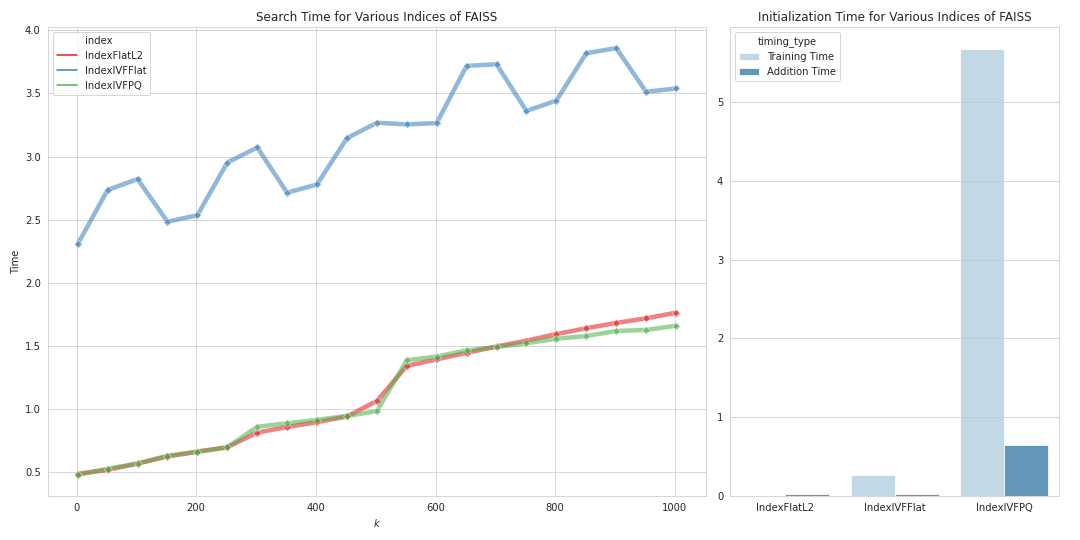
\includegraphics[width=0.85\linewidth,height=0.65\textheight]{../images/knn/timings}
\caption{Timings for $k$-NN graph construction (query time on the left-hand side, index training and point addition time on the right-hand side) on Oxford105K data set. It is clear that, in terms of time, \texttt{faiss} powered by GPU outperforms KGraph \cite{Dong2011} we experimented with before (recall that it took KGraph approx. 105s to finish the search for 100 nearest neighbors).}
\label{fig:knn_timing}
\end{figure}
\end{frame}


\subsection{Precision Evaluation}


\begin{frame}

\begin{figure}
\centering
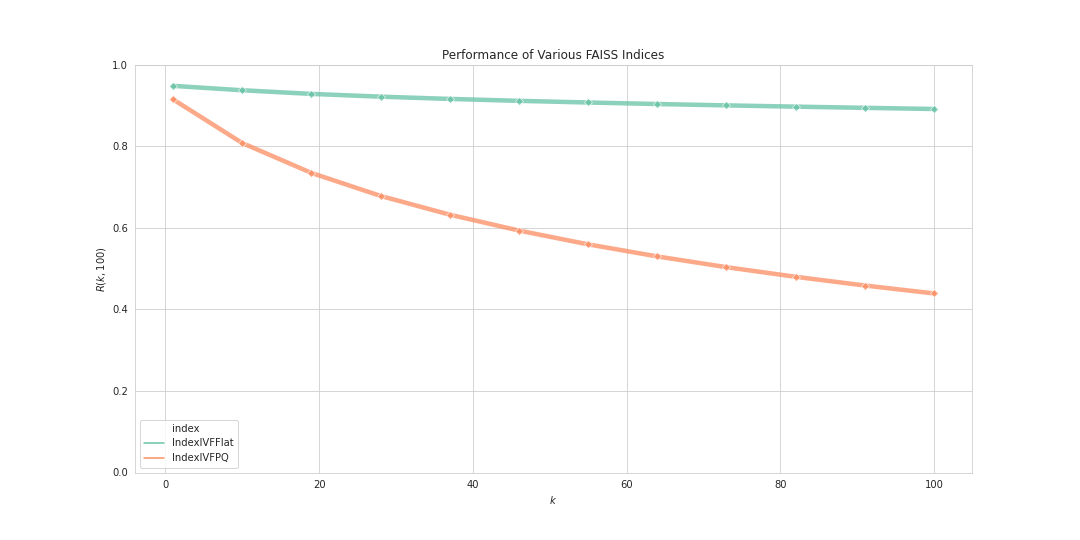
\includegraphics[width=0.85\linewidth,height=0.65\textheight]{../images/knn/precision}
\caption{$R(k, 100)$ measured for \texttt{IndexIVFFlat} and \texttt{IndexIVFPQ} on Oxford105K data set.}
\label{fig:knn_precision}
\end{figure}
	
\end{frame}


\subsection{Smooth $k$-NN Graph Paths}


\begin{frame}
\begin{block}{Smooth Path Evaluation}
	Another exercise we have performed in the scope of this work is the implementation of the path search given by equation (12) in \cite{Johnson2017}. We have utilized a depth-first search with a cut-off to generate simple paths in the k-NN graph. To stress the preference on path smoothness, the choice of the final path was made according to cost function $\min_{P} max_{i} d_{p_{i}, p_{i+1}}$ where $P = (p_{1}, p_{2}, \dots, p_{n})$ denotes paths between the source and the target and $n <$ cut-off value. If more than one paths can be chosen, the shortest one of the remaining is picked. An example is shown in Fig.~\ref{fig:smooth_path}.
\end{block}

\end{frame}


\begin{frame}

\begin{figure}
\centering
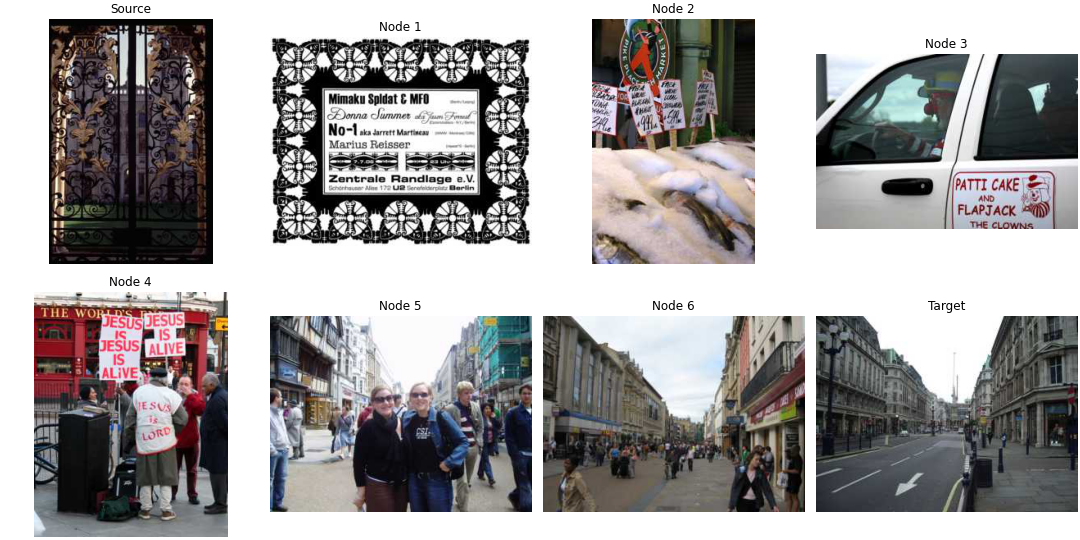
\includegraphics[width=0.85\linewidth,height=0.65\textheight]{../images/knn/path}
\caption{Sample of the smooth path search between the source image and the target image within the exact 10-NN graph of the whole Oxford105K data set; the cut-off value was set to 7.}
\label{fig:smooth_path}
\end{figure}

\end{frame}